\chapter{Classi deterministiche di complessità}

\section{Macchine di Turing}

La macchina di Turing è un celebre modello di calcolo introdotto in \ref{sec:turingmachine}. Lo
rivediamo qui per comodità in una versione leggermente diversa (multi-tape).

\begin{defn}
    Una Macchina di Turing (multi-tape, deterministica) è una tupla $\tuple{Q, \Gamma, b, \Sigma,
    k, \delta, q_{0}, F}$ dove
    \begin{itemize}
        \item $Q$ è un insieme finito di stati
        \item $\Gamma$ è l'alfabeto finito del nastro
        \item $b$ è il carattere bianco
        \item $\Sigma \subseteq \Gamma \setminus \set{b}$ è l'insieme dei caratteri di input/output
        \item $k \geq 1$ è il numero di nastri
        \item $q_{0} \in Q$ è lo stato iniziale
        \item $F \subseteq Q$ è l'insieme degli stati finali (o di accettazione)
        \item $\delta: Q \setminus F \times \Gamma^{k} \to Q \times \Gamma^{k} \times
        \set{L,R}^{k}$ è la funzione di transizione.
    \end{itemize}
\end{defn}

Intuitivamente abbiamo una serie di nastri con memoria illimitata, divisi in celle di dimensione
fissata. Ogni cella può contenere un carattere di un alfabeto dato, compreso un carattere $b$
(bianco) di inizializzazione. Abbiamo una testina mobile di controllo per ogni nastro ed un automa
di controllo a stati finiti.

Le operazioni fondamentali sono la lettura o scrittura di caratteri individuati dalla testina, lo
spostamento della testina verso destra o verso sinistra, e la modifica dello stato interno
dell'automa.

Per le misure di complessità in genere si tende sempre a prendere come riferimento la macchina di
Turing. Questo perché con questo modello di calcolo sono ben chiari i concetti di unità di tempo e
di unità di spazio, che corrispondono rispettivamente ad una transizione e ad una cella di memoria.
Ci chiederemo quanti nastri ci permettiamo di usare. Vedremo che questo farà la differenza.

I nastri sono infiniti, ma in ogni momento si suppone che solo una parte finita del nastro sia stata
scritta. I nastri partono blank, su di essi viene scritto l'input e su di essi si svolge la
computazione.

È la funzione di transizione che governa il comportamento della macchina.

\subsection{Convensioni di input output}

Slide 47

Si suppone in genere di avere un nastro di input sul quale possono essere effettuate solo letture e
ci si può muovere in una sola direzione. Non è limitante dato che possiamo sempre copiare il
nastro di input in un nastro di lavoro e fare quello che vogliamo sul nastro copia.

Abbiamo anche un nastro di output, di sola scrittura, la cui testina avanza in una sola direzione.

Si suppone in genere di avere già l'input su nastro prima di cominciare la computazione.  Questa
ipotesi non cambia le considerazioni già fatte sulle complessità sublineari, in genere poco
interessanti. Per convenzione supponiamo che la computazione cominci con la testina sul primo
carattere dell'input, con le altre celle che hanno il carattere blank.

Per convenzione supponiamo che, alla fine della computazione, l'output sia la più lunga stringa di
caratteri dell'alfabeto non blank alla sinistra della testina del nastro di output.

È importante non confondere configurazione iniziale e stato iniziale.

\subsection{Configurazioni}

Una configurazione è una descrizione dello stato della computazione ad un dato istante della
computazione.

Rappresentiamo le configurazioni mediante tuple così fatte:
\begin{equation*}
    q, (\sigma_{1},\tau_{1}),\dotsc,(\sigma_{k},\tau_{k})
\end{equation*}
dove $q$ è lo stato dell'automa e $\sigma_{i}$ e $\tau_{i}$ sono due stringhe di caratteri che
descrivono la porzione non (definitivamente) bianca del nastro $i$ alla sinistra e alla destra della
relativa testina. Il carattere in lettura è il primo carattere di $\tau_{i}$.

La computazione avviene per passi discreti: una transizione tra due configurazioni è una relazione
$\vdash$ governata dalla funzione di transizione:
\begin{equation*}
    (q,(\sigma_{1}b_{1},a_{1}\tau_{1}),\dotsc,(\sigma_{k}b_{k},a_{k}\tau_{k})) \vdash
    (q',(\sigma_{1}\beta_{1},\alpha_{1}\tau_{1}),\dotsc,(\sigma_{k}\beta_{k},\alpha_{k}\tau_{k}))
\end{equation*}
se
\begin{itemize}
    \item $\delta(q,a_{1},\dotsc,a_{k}) = (q',a_{1}',\dotsc,a_{k}',D_{1},\dotsc,D_{k})$
    \item se $D_{i} = R$, allora $\beta_{i} = b_{i}a_{i}'$ e $\alpha_{i} = \varepsilon$
    \item se $D_{i} = L$, allora $\beta_{i} = \varepsilon$ e $\alpha_{i} = b_{i}a_{i}'$
\end{itemize}

La relazione $\vdash^{*}$ denota la chiusura transitiva e riflessiva della relazione $\vdash$.

\begin{defn}
    Una funzione $f: \Sigma^{*} \to \Sigma^{*}$ è calcolata da una macchina di Turing $M$ se per
    ogni $\alpha$ esiste $q_{f} \in F$ tale che
    \begin{equation*}
        q_{0}, (\varepsilon,\alpha),\dotsc,(\varepsilon,\varepsilon) \vdash^{*} q_{f},
        (\gamma_{1},\tau_{1}),\dotsc,(\gamma_{k},\tau_{k})
    \end{equation*}
    e $f(\alpha)$ è il più lungo prefisso di $\gamma_{k}$ appartenente a $\sigma^{*}$
\end{defn}

Detto in altri termini una computazione parte dallo stato iniziale, con i nastri vuoti, con l'input
sul nastro di input e procede per configurazioni succesive, fino ad arrivare ad una configurazione
finale (se la funzione calcolata è definita per il dato input).

\begin{equation*}
    \overequalto{c_{0}}{\varepsilon,q_{0},x} \to c_{1} \to c_{2} \to \cdots \to c_{F}
\end{equation*}

Dato che in complessità noi consideriamo problemi decisionali di solito l'output non è
interessante di per sè. Potremmo avere due stati interessanti, uno di accettazione e uno di
rifiuto.

Nel modello deterministico l'evoluzione della macchina è completamente determinata e univoca per la
macchina considerata dato lo stato iniziale. Lo schema è lineare. La macchina non deterministica
invece non ha una sola mossa disponibile, ne ha un set. Ci possono essere più scelte riguardo alla
mossa successiva.

Lo schema corrispondente smette di essere una sequenza e diventa un grafo, come si puo notare in
figura \ref{img:nondetcomp}.

\begin{figure}[h]
    \begin{center}
        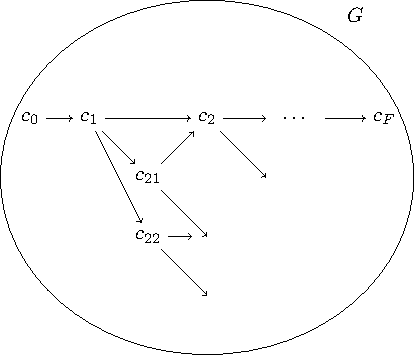
\includegraphics{img/NonDetComputation.pdf}
        \caption{Schema di una computazione non deterministica}
        \label{img:nondetcomp}
    \end{center}
\end{figure}

La computazione della macchina deterministica è un grafo con milioni di nodi. Inoltre questi nodi
sono ``grossi'', un sacco di informazione è codificata in ogni nodo. Questo è un esempio vero di
grafi ``grossi'' (Internet a confronto è un grafo piccolo).

Questo è fondamentale per quanto riguarda la simulazione deterministica della macchina non
deterministica. Fondamentalmente questo si riduce a visitare tutti i cammini del grafo della
computazione della macchina non deterministica.

Il problema è che dobbiamo visitare tutti i cammini del grafo. Solitamente non basta una visita
semplice. Abbiamo il problema di come svolgere questo processo. Lo rivedremo più avanti.

\section{Classi di complessità}

Prima di vedere le classi di complessità definiamo un pò di operazioni: $\textit{time}_{M}$,
$\textit{space}_{M}$, $t_{M}$, $s_{M}$.

\begin{defn}
    Sia $M$ una Macchina di Turing.
    \begin{itemize}
        \item $\textit{time}_{M}(x)$ è il tempo di esecuzione di $M$ su input $x$: il numero di
        passi richiesti per la computazione
        \item $\textit{space}_{M}(x)$ è il numero massimo di celle visitate da una qualche testina
        durante la computazione (per macchine a più nastri si considerano solo i nastri di lavoro)
        \item $t_{M}(n) := \max\set{\textit{time}_{M}(x) \mid |x| = n}$
        \item $s_{M}(n) := \max\set{\textit{space}_{M}(x) \mid |x| = n}$
    \end{itemize}
\end{defn}

Se in una computazione abbiamo una configurazione $\tuple{\beta, q, \alpha}$ su qualche nastro dove
la lunghezza di $\beta$ e $\alpha$ sono massime, lo spazio consumato è uguale alla somma tra la
lunghezza di $\beta$ e $\alpha$.

Le prime due funzioni calcolano la complessità in funzione dell'input, ma noi vogliamo calcolarla
in funzione della dimensione dell'input. Definiamo quindi le altre due operazioni. $t_{M}$
rappresenta il caso pessimo di complessità in tempo per stringhe di lunghezza $n$. $s_{M}$ è un
analogo per lo spazio.

\begin{defn}
    Sia $f:\Nat \to \Nat$. Definiamo le seguenti classi di complessità:
    \begin{itemize}
        \item $\DTIME(f) := \set{\Lang \subseteq \Sigma^{*} \mid \exists M, \Lang = \Lang_{M} \land
        t_{M} \in O(f)}$
        \item $\DSPACE(f) := \set{\Lang \subseteq \Sigma^{*} \mid \exists M, \Lang = \Lang_{M} \land
        s_{M} \in O(f)}$
    \end{itemize}
\end{defn}

Le classi di complessità sono classi definite in termini di funzioni. La funzione di input mi dà
un ordine di grandezza, non una misura precisa. In altre parole sia interessati ad $O(f)$.

\textbf{Nota bene:} le classi \textbf{non rappresentano tempi o spazi}. Rappresentano classi di
problemi, o, più formalmente, insiemi di linguaggi.

$\DTIME(f)$ rappresenta l'insieme di linguaggi che sono accettabili da una macchina di Turing in un
tempo $O(f)$.

$f$ è una funzione della dimensione dell'input. $\DTIME(n^{2})$ è l'insieme dei linguaggi che sono
riconosciuti da una MdT in tempo quadratico.

\section{Relazione tra spazio e tempo}

Il teorema che vediamo ora è molto importante. È analogo, a livello di importanza, al problema
della terminazione della teoria della calcolabilità. Ci dice qualcosa sulla relazione tra
complessità in tempo e complessità in spazio.

Sapendo che un certo linguaggio ha una certa complessità in tempo posso dire qualcosa sulla sua
complessità in spazio, e viceversa?

Partiamo dalla parte più facile. Supponiamo di avere la complessità in tempo di un algoritmo.

Che motivazioni abbiamo per voler sapere la complessità in tempo? Una è sicuramente che il tempo
è una risora critica. Inoltre è una misura più fine di quella di spazio, ci dà un upper bound
allo spazio. Questo perché se voglio aumentare l'occupazione di spazio, con la MdT, devo scrivere
nuove celle. Sporcare una nuova cella richiede almeno un'unità di tempo. La complessità in tempo
dà un upper bound stretto alla complessità in spazio.

Questo è importante, ed è anche una delle ragioni per cui il tempo è più interessante dello
spazio.

Questo discorso vale a meno di costanti, dato che definiamo noi l'unità di tempo e spazio. Ma una
volta definite queste il discorso resta immutato.

Abbiamo quindi che $\DTIME(f) \subseteq \DSPACE(f)$. A prima vista sembrerebbe un'``inversione''. In
realtà se ci pensa se abbiamo un upper bound alla complessità in tempo richiesta per risolvere un
problema abbiamo che lo stesso upper bound si applica per la complessità in spazio, e quindi i
linguaggi di $\DTIME(f)$ fanno sicuramente parte di $\DSPACE(f)$.

\begin{thm}
    Sia $f: \Nat \to \Nat$. Allora $\DTIME(f) \subseteq \DSPACE(f)$.
\end{thm}
\begin{proof}
    Supponiamo che $\Lang \in \DTIME(f)$. Abbiamo quindi che $\exists M, \Lang = \Lang_{M} \land
    t_{M} \in O(f)$. Ma se $t_{M} \in O(f)$ allora anche $s_{M} \in O(f)$. Questo perché il tempo
    è un upper bound allo spazio. Ma quindi $\Lang \in \DSPACE(f)$.
\end{proof}

La D sta per deterministic in queste due classi sta per determinstic.

Per dimostrare il teorema abbiamo svolto la nostra analisi sulla stessa macchina. Questo non è
richiesto per la dimostrazione, dato che potrei immaginare di svolgere la dimostrazione con un'altra
macchina per la parte della complessità in spazio. In questo caso non è stato necessario, il
teorema è puntuale sulla macchina. Se una certa macchina ha una certa complessità in tempo ha la
stessa complessità, al più, in spazio.

Si può occupare anche meno spazio, il tempo fa da upper bound.

Questa era la parte facile, ragioniamo ora sul viceversa. Data la complessità in spazio posso dire
qualcosa sulla complessità in tempo?

Supponiamo ad esempio che una certa macchina di Turing lavori in spazio costante. Quando misuriamo
la complessità in spazio di solito abbiamo macchine multinastro. Di solito non consideriamo lo
spazio del nastro di input. Noi consideriamo solo lo spazio aggiuntivo di cui la macchina ha bisogno
per svolgere la computazione.

In questo ha caso ha senso parlare di complessità sublineari, dato che magari non abbiamo bisogno
di uno spazio aggiuntivo della stessa dimensione dell'input. In particolare possiamo avere spazio
costante, indipendente dall'input.

Un punto importante è che la complessità la misuriamo sempre al termine della computazione. Se la
computazione non termina la complessità è indefinita, quindi non è un caso interessante quello di
loop infinito. Se la complessità è definita non possiamo divergere.

Siamo in loop se passiamo per due volte sulla stessa configurazione. Ma noi questo non lo
permettiamo. Perciò abbiamo un insieme finito di possibili configurazioni che verranno assunte in
una computazione che giunge a termine.

Proviamo a calcolare il numero possibile di configurazioni immaginando di lavorare con uno spazio
costante. Consideriamo i possibili nastri diversi di lunghezza $L$. Questi sono $|\Sigma|^{L}$.
Moltiplichiamo per $|Q|$, il numero di stati. Infine moltiplichiamo per $L$, dato che la testina
potrebbe essere su qualsiasi cella del nasto. Otteniamo la seguente quantità:
\begin{equation*}
    L \times |Q| \times |\Sigma|^{L}
\end{equation*}

Questo rappresenta un upper bound alla complessità in tempo del problema.

Il numero degli stati è fissato in base alla macchina. L'ordine è dato da $L$. La crescita è
esponenziale. Non è così grave, c'è molto di peggio.

Questa analisi vale in caso di complessità costante. Cambia qualcosa se la complessità in spazio
ha un ordine $O(s(n))$? No, basta che la mia $L$ diventi una $L(s(n))$. Il discorso si applica
invariato. Sappiamo che o la macchina termina entro questo upper bound oppure è in loop.

Anche qui l'analisi è puntuale. Data una macchina e una complessità in spazio posso dare una
complessità in tempo sulla stessa macchina, non ne devo produrre un'altra.

In un certo senso per alcuni programmi non possiamo decidere la terminazione perché non possiamo
neanche decidere la quantità di spazio che verrà richiesto. Si può dimostrare che se è
decidibile il problema di sapere qual è l'occupazione di una certa risora saprei qualcosa riguardo
le altre risorse. Questo perché tutte le misure di complessità sono correlate. Questa correlazione
può essere pessima a piacere, nel nostro caso era esponenziale.

In questa analisi stiamo dimenticando qualcosa. Sembrerebbe che se abbiamo una complessità in
spazio costante avremmo una complessità in tempo costante, e quindi sublineare. Tuttavia in realtà
noi dobbiamo sapere anche fino a che punto siamo arrivati nell'input. Questo va ad influire sul
numero delle combinazioni. In particolare va aggiunta la lunghezza dell'input alla misura data
prima.
\begin{equation*}
    n*L \times |Q| \times |\Sigma|^{L}
\end{equation*}

Quindi abbiamo che, se $M \in \DSPACE(f(n))$ allora $\exists c, M \in \DTIME(c^{f(n) + \log(n)})$.
Ricordiamo che $n = c^{\log(n)}$.

\begin{thm}
    Sia $f: \Nat \to \Nat$. Allora $\DSPACE(f) \subseteq \bigcup_{c \in \Nat}\DTIME(c^{log + f})$.
\end{thm}

Ancora una volta l'esponenziale non è così male. Tutta la teoria della complessità si gioca tra
esponenziale e polinomiale, è un vincolo abbastanza vicino.

\section{Dipendenza dal modello di calcolo}

La macchina di Turing è molto flessibile dato che ci sono tante variabili che possono influire. Ci
chiediamo quanto questo ci influenzi nella nostra analisi.

Se rimpiccioliamo l'alfabeto abbiamo bisogno di stati nuovi per ricordare che ruolo ha un simbolo del
nuovo alfabeto rispetto a quello che aveva nel vecchio.

Lo slowdown è lineare. Se passiamo, ad esempio, da ASCII a binario dovremo fare 8 passi per uno
equivalente. Era di moda tempo fa la ricerca della macchina di Turing universale che minimizzasse la
somma tra grandezza dell'alfabeto e numero di stati.

Vediamo qualcosa di più importante, ovvero la riduzione dei nastri.

Immaginiamo di passare da due nastri ad un solo nastro. Perché è problematico lavorare con un
nastro? Immaginiamo di avere una stringa $l$ sul nastro e di volerla copiare più avanti. Con un
nastro solo questa operazione è molto complessa. Dobbiamo leggere i caratteri $x_{0},\dotsc,x_{n}$
uno alla volta, memorizzando il carattere con uno stato interno. Non possiamo memorizzare l'intera
stringa usando uno stato interno perché non abbiamo un upper bound alla lunghezza della stringa.

\begin{figure}[h]
    \begin{center}
        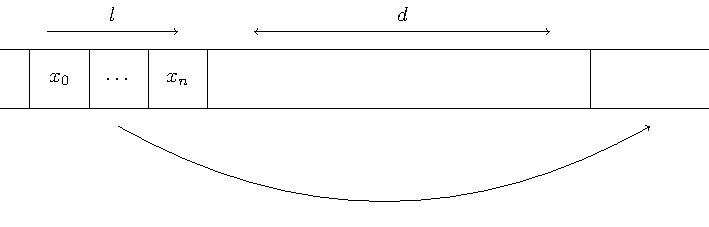
\includegraphics{img/CopyString.pdf}
        \caption{Copia di una stringa con due nastri}
    \end{center}
\end{figure}

Se la distanza è $d$ sono necessari $d\cdot l$ giri avanti e indietro. Essendo $d$ almeno lineare in $l$
(non consideriamo condizioni di overlap) abbiamo complessità almeno quadratica.

Con due nastri è semplice. Basta copiare la stringa di input su un altro nastro, posizionare la
testina del nastro di input dove vogliamo copiare la stringa e posizionare la testina del secondo
nastro all'inizio della stringa. A questo punto è sufficiente scrivere nel primo nastro il
carattere letto dalla testina sul secondo nastro fino a raggiungere la fine della stringa.

\begin{figure}[h]
    \begin{center}
        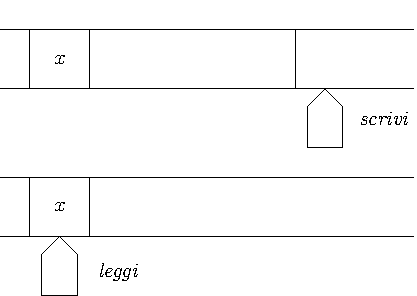
\includegraphics{img/CopyString2Tapes.pdf}
        \caption{Copia di una stringa con due nastri}
    \end{center}
\end{figure}

Passando da due nastri ad uno abbiamo uno slowdown che può essere quadratico. Questo è pesante. La
complessità computazionale dipende dal modello di calcolo. Nell'ambito delle macchine di Turing
questi slowdown restano però polinomiali.

C'è una sottigliezza da considerare riguardo la macchina a due nastri. Le due testine possono
essere lontane a piacere, e il tempo di trasmissione tra le due può quindi aumentare
arbitrariamente. Non è sempre corretto considerare il costo della tramsissione pari ad 1.
